\documentclass[12pt,letterpaper]{article}
\usepackage{fullpage}
\usepackage[top=1.5cm, bottom=4.5cm, left=2cm, right=2cm]{geometry}
\usepackage{amsmath,amsthm,amsfonts,amssymb,amscd}
\usepackage{lastpage}
\usepackage{enumerate}
\usepackage{enumitem}
\usepackage{fancyhdr}
\usepackage{mathrsfs}
\usepackage{xcolor}
\usepackage{verbatim}
\usepackage{graphicx}
\usepackage{listings}
\usepackage{hyperref}
\usepackage{sidecap}
\usepackage{lipsum}
\usepackage{multicol}
\usepackage{csquotes}
\usepackage{authblk}

\hypersetup{
  colorlinks,
  citecolor=false,
  linkcolor=false,
  urlcolor=false}
\usepackage{subfiles}
\usepackage{subfigure}

% Bibliography Packages
\usepackage[utf8]{inputenc}
\usepackage[english]{babel}
%\usepackage{biblatex}
\usepackage[
    backend=biber,
    style=alphabetic,
  ]{biblatex}
\addbibresource{Bibliography.bib}


\hypersetup{%
  colorlinks=true,
  linkcolor=black,
  linkbordercolor={0 0 1}
}
 
\renewcommand\lstlistingname{Algorithm}
\renewcommand\lstlistlistingname{Algorithms}
\def\lstlistingautorefname{Alg.}

\lstdefinestyle{Python}{
    language        = Python,
    frame           = lines, 
    basicstyle      = \footnotesize,
    keywordstyle    = \color{blue},
    stringstyle     = \color{green},
    commentstyle    = \color{red}\ttfamily
}

%\setlength{\parindent}{0.35in}
\setlength{\parindent}{0pt}
\setlength{\parskip}{0.15in}

% Edit these as appropriate
\newcommand\NetIDa{Chang, Dunham, Kallepalli, Khalil, Kim, Kwan, Leung}
\newcommand\NetIDb{Group 10}


\pagestyle{fancyplain}
%\headheight 14pt
%\lhead{\NetIDa}
\lhead{\NetIDa}                
\rhead{\thepage   }
%\lfoot{}
\cfoot{}
%\rfoot{\small\thepage}
\headsep 3em


\linespread{1.5} 
\begin{document}

\begin{titlepage}
   \begin{center}
       \vspace*{.5cm}

       \textbf{Stats 141XP Final Report:}

       \vspace{.1cm}
        \textbf{Variable Design and Analysis for UCLA Extension Programs}
            
       %\vspace{.5cm}
    \textbf{Group 10}
    
       \textbf{Allan Chang, Joseph Dunham, Ajay Kallepalli,\\
       Yonatan Khalil, Daniel Kim, Jason Kwan, Kyle Leung}
       
       %\vspace{.1cm}
       
       
       \vspace{1cm}
     
            
       Department of Statistics, UCLA\\
       Professor Esfandiari\\
       June 11, 2021\\
          
          \vspace{1cm}
          {\large\textbf{Abstract}\par}  
   \end{center}

\vspace*{-5mm}

\noindent
The overall objective of our study was to use data to understand "What motivates students to come to study at the ALC?" The data we were given included the anonymized survey data, letter grade, and demographic data of students. 

Given the data and the objective our group focused on three areas. The first aimed to find the best predictors of program success, the second was to understand students' elective choice preferences, and the third was to try to quantify the level of engagement of students. Due to the varied nature of both the predictor and response variables in the dataset multiple statistical methods were necessary for analysis. To identify predictors of program outcomes for questions one and two, multiple linear regression, logistic regression, and sentiment analysis were used. The third question used factor analysis, AIC/BIC Criterion, and post-hoc analyses to identify the most significant predictors.
From our statistical analyses we found that region was significant in predicting course outcomes and elective preferences, further the same students are more likely to be attracted to cu \end{titlepage}-ltural, test prep, and business English courses. Age and whether a student failed a class or not was also related to the likelihood of them signing up for a test prep class. These results were all statistically significant to the 95\% confidence level. With regards to predicting engagement we found the following variables to be statistically significant: placement levels, new vs returning students, Payor, how they heard about ALC, planned field of study, and AEIP completion.

The main challenges faced were in working with and cleaning the multiple disparate data files in order to make a unified dataset. Potential next steps include analyzing the demographics of those students that are most or least engaged. We also recommend potential changes to the survey design in order to encourage better survey responses which could help with further analysis, particularly sentiment analysis.


%\thispagestyle{empty}
%\clearpage

\setcounter{page}{1}


%%START REPORT%%
%***INTRO***%
\section{Statement of the three problems}
What demographic and academic variables best account for program outcomes?
%\vspace*{-5mm}
\begin{itemize}
\setlength\itemsep{.1mm}
\item Here program outcomes were taken to be letter grades, pass/no pass, absences, and student evaluations.
\item Enables better identification of the behaviors of good and bad students, which will allow ALC to promote positive behaviours and discourage negative ones. 
\item Ultimately the goal is to improve the learning experience of students who are enrolled in ALC and UCLA Extension. 
\end{itemize}
What are the patterns in students’ elective preferences and overall academic performance?
\begin{itemize}
\setlength\itemsep{.1mm}
\item Useful to ascertain how students choose electives and if there's any relationship between the electives students choose. 
\end{itemize}
What are the best variables that help us quantify and predict the engagement of students?
\begin{itemize}
\setlength\itemsep{.1mm}
\item Helps to identify those groups of students that are most engaged in order to maximize the marketing efforts of the ALC and UCLA Extension program towards those that will receive the most benefit. 
\item An additional benefit could be to increase diversity of student groups that show high engagement but are relatively underrepresented.
\end{itemize}


%***Data***%
\section{Data}

\subsection{Files}

The data folder used for this study was sourced from the UCLA Extension’s Academic Intensive English Program, or AIEP, and can be split into seven types of files; all file types include a student’s ID and quarter. Also, because the survey questions changed in content or number per quarter or year, the files included in each type generally increase in their number of columns.

The first file type, essentially notated as Dashboard, has only one file and records student demographic information and student statuses; however, much of the demographic information can also be found repeated in the other file types. The second file type, Elective Preferences, has twelve files and records student course choices for intermediate and advanced courses as well as their plans for the directly subsequent quarters. The third file type, Enrollment, has four files and re-records some of the student demographic information and also includes their visa, major, and English skill levels in various aspects, including grammar, reading, and speaking. The fourth file type, Market, has three files and records students’ personal and life profiles, including their pre-program history, their post-program plans, how they pay for the program, how they stay in touch with family and friends, and the English tests in their past and future. The fifth file type, Placement, has three files and records student English skill levels, especially as found using the Oxford Placement Test. The sixth file type, Placement Finals, has two files and records course and section number, course title, teacher, some demographic information, absences, grades, and English skill level. The seventh file type, Program Evaluations, includes eight files and records student evaluations of their teachers, courses, and course aspects such as teacher organization, chances to participate in class, and satisfaction with course textbook and course materials; the latter half of the six files also contain multiple choice and free response questions related to satisfaction of students’ self-gauged improvements and satisfaction with various non-academic aspects of the AEIP, including counseling, staff, and tours.

\subsection{Final Variables}

All variables can generally be split into three types: string, numeric, and categorical. The only example of a string variable for this study is Student ID; Student ID needed to be kept identical between sets in order to properly compare and merge data frames based on the IDs. The best example of a numeric variable for this study is birth year. Lastly, a good example of a categorical variable for this study is ZIP code; as stated before, the vast majority of categorical variables needed to be re-coded for legibility and ease of interpretation.

In file type Dashboard, the final columns kept were birth year, gender, country of citizenship, preferred ZIP code, payor, and new or returning student status; almost all redundant demographics columns in the other file types were also removed.

In file type Elective Preferences, for both intermediate and advanced electives the only columns kept were first and second choice of course for the schedule pairs Monday-Wednesday and Tuesday-Thursday; the columns recording plans to study in the AEIP during the next quarter and desire for 4-day test prep were dropped, first because they were directly mirrored in terms or responses, i.e. any student who gave an answer for AEIP did not give one for test prep, and second, because it was found that all responses for AEIP were Yes and therefore could not have any statistical significance.

In file type Enrollment, the final columns kept were birth year, gender, country of citizenship, preferred ZIP code, sponsor, payor, new or returning student status, initial placement by ALC, ALC education level cohort, multiple English skill variables, and program completion status. The demographics columns were kept to identify students if the enrollment dataset were merged without also including Dashboard. The columns for visa, major, and prior skill levels were found to lack statistical significance or were too sparsely populated with values, and thus were removed.

In file type Market, the final columns kept were pre-program history, post-program life plans, payor, how the student heard about the program, any student-owned devices, the student’s means of social contact, the student’s six-month history of and six-month plans for any English tests, and the student’s planned major or field of study. The two columns removed were level and previous English test score; the former holds no values at all and the latter would be redundant.

In file type Placement Finals, the final columns kept were instructor name, course ID, log-transformed absences, final course grade, and course level; all other columns recorded either redundant information, including demographics and course information, or course’s campus location.

In file type Program Evaluations, the final columns kept were all course evaluation columns, all student-gauged improvement columns, and all multiple-choice satisfaction or query columns; essentially, all removed columns were those that could not be cleanly or simply converted into a categorical variable.

\subsection{Schematics}

\begin{center}
    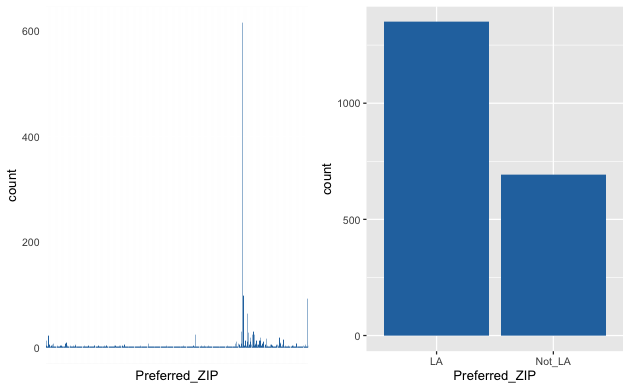
\includegraphics[scale = 0.5]{Plots/schematic1.png}
\end{center}

The above figure displays preferred ZIP code, sourced from Dashboard, both as recorded by students and as re-coded for the study. Preferred ZIP code had a very large number of unique values and thus was hard to read and interpret; all values were consequently re-coded to either LA or Not LA, with LA zip codes being all values between 90001 and 93951 inclusive; interestingly, the tallest bars in the first plot actually match to LA zip codes.

\begin{center}
    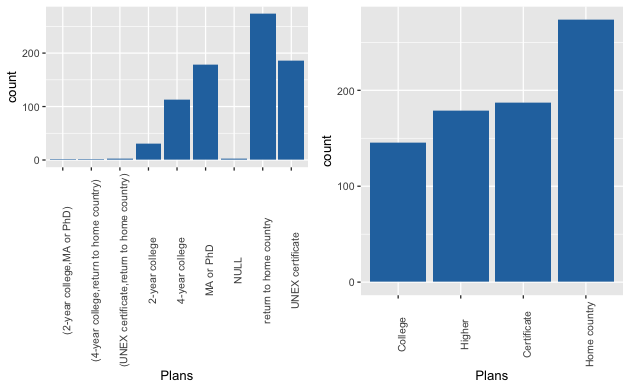
\includegraphics[scale = 0.5]{Plots/schematic2.png}
\end{center}

The above figure displays student plans after the program, sourced from Market. Again, the variable had too many unique values to be worth interpreting or to be valuable in interpretation at all; thus, all values were re-coded to College, Higher, Certificate, and Home country based on their first listed element.

\begin{center}
    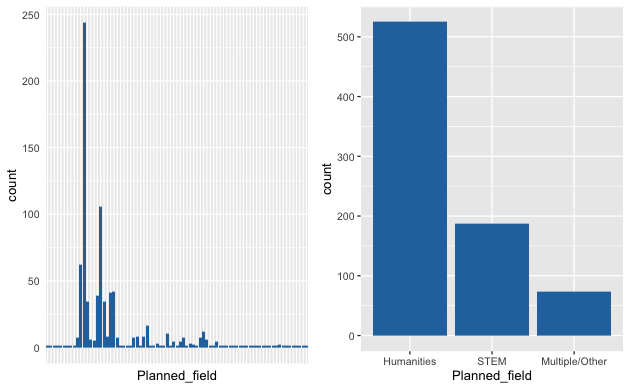
\includegraphics[scale = 0.5]{Plots/schematic3.png}
\end{center}

The above figure displays the students' planned majors or field(s) of study, again sourced from Market. The two highest values in the first plot are respectively Business/Finance and Engineering, which contribute greatly to their columns in the second plot, Humanities and STEM, respectively. Multiple/Other records any students who had multiple majors listed or alternatively did not list any plans or fields.

\subsection{Process}

After examining and stepping through the data files to understand what each of them represented and included, cleaning the provided data required finding and solving any universal issues within the dataset; in this case, there were five main universal issues found and solved. First, multiple files had repeated data; this list included three files from Enrollment and one from Program Evaluations. Second, virtually every dataset included null ID observations that required removal, as null ID observations could not be used to identify any students within or between datasets and most likely were due to students’ clerical errors or survey system errors.

The next portion of the process required determining which variables (excluding student ID and quarter as main identifiers of person and time) and observations should be kept and changed to overall simplify the data. This effort also was intended to make each of the data file types uniform in number and type of variables and therefore mergeable between files of the same type or of different data types. Stemming from this, the third issue was to remove any columns recording redundant demographics as well as what year, time, and collector the students’ responses were recorded from. The fourth issue to solve with the data was to recode most variable names and categorical variable values to ease future code and interpretation. For example, many survey questions were directly used as variable names and column headers, and thus needed to be abbreviated or renamed for legibility. Another example is student payor values from Dashboard, which included unnecessary seven-character code endings. The third and likely best example is all of the multiple choice survey questions in the program evaluations, which required being re-coded from degree-of-satisfaction values to numbers to be summed and evaluated later.

The fifth and final issue during this process was determining what to do with quarter data, as the way quarters were recorded or encoded varied between data file types; eventually, the final decision was made to recode all quarters to only the last two digits of the quarter’s year and which quarter in the year it was (ex. "AEIP Summer 2016 2nd Half" to "16SU").

\newpage

%***Demographics and Preferences***%
\section{Demographics and Preferences}

There were three primary questions that we sought out to answer that relate to demographics and preferences.

\begin{itemize}
    \item What patterns can be found in students who left good/bad course reviews?
    \item What patterns can be found in student elective preferences?
    \item Which demographic and academic variables best account for program outcomes?
\end{itemize}

\subsection{Sentiment Analysis}

A sentiment analysis was performed on the free-response data gathered from the course and teacher reviews. To facilitate this, reviews were combined by student, of which there were 472 who submitted at least one review. The AFINN Lexicon, an open-source database, was used to generate the sentiments. Each word was assigned a value, with positive values corresponding to positive words and negative values to negative words, and each student was scored by the sum of their sentiment values.

\begin{center}
    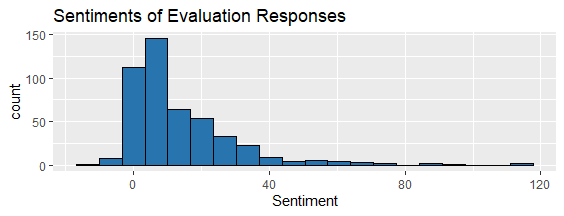
\includegraphics{Plots/sentiment_hist.png}
\end{center}

\newpage

We can see the cloud of words that were considered below. The majority of words are associated with a sentiment value of 0. Common grammatical words (e.g. "the") were removed.

\begin{center}
    
\includegraphics{Plots/full_cloud.png}
\end{center}

Also plotted are word clouds of the words used that yielded positive responses and negative responses separately. Note that the scales are unequal, as positive words were used more often.

\begin{figure}[!bp]
  \centering
  \begin{minipage}[b]{0.4\textwidth}
    
\includegraphics[width=\textwidth]{Plots/good_cloud.png}
    \caption{Positive Values}
  \end{minipage}
  \hfill
  \begin{minipage}[b]{0.4\textwidth}
    
\includegraphics[width=\textwidth]{Plots/bad_cloud.png}
    \caption{Negative Values}
  \end{minipage}
\end{figure}

\newpage

Attempts to find patterns in course results based on student sentiment were unsuccessful. There is no connection between student sentiment and course result. In addition, there is also no connection between the length of review and course result.

\begin{center}
    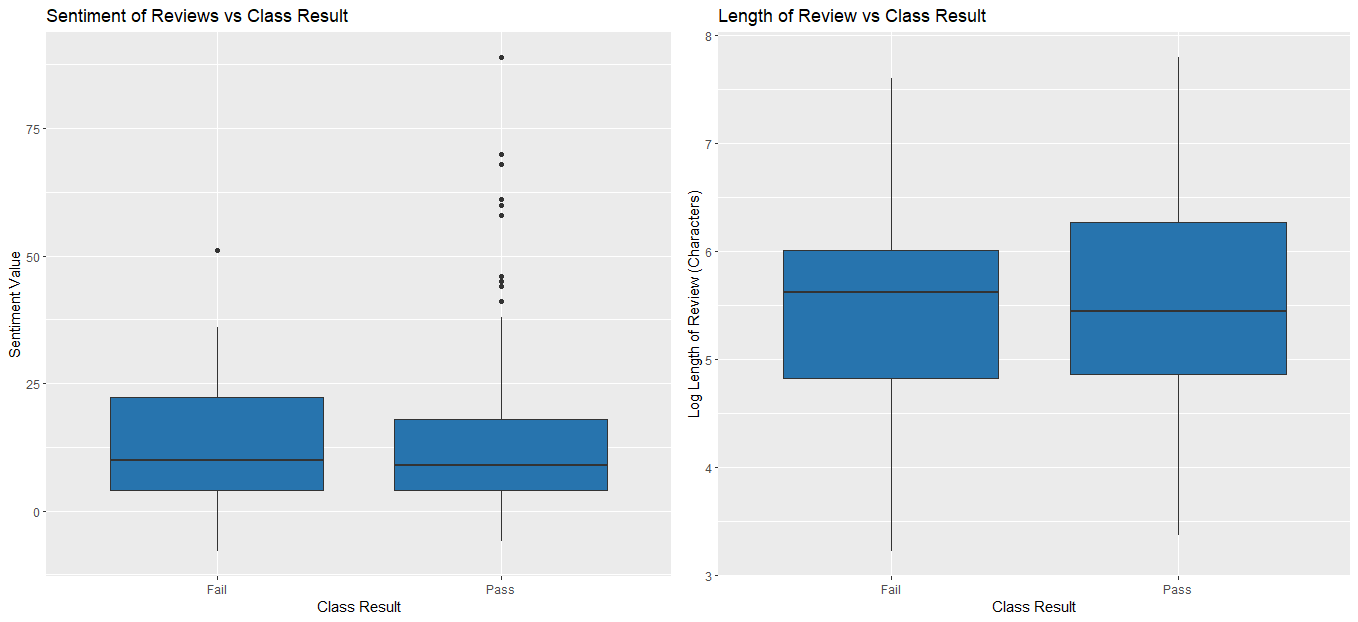
\includegraphics[width = \textwidth]{Plots/sentiment_boxes.png}
\end{center}

There are a number of potential reasons for this. The sample size of students that have both course results data and at least one review is fairly small (221 students), and many reviews that were available contained very little information. In addition, negative responses may be more likely to be suppressed by the nature of a voluntary review, as well as suppressed by the sentiment analysis when complaints are formulated as suggestions (e.g. the book should be newer). Furthermore, sentiment analysis may be more difficult to apply to English-learners, whose word choice may not be in line with native speakers.

%%%%%%%%%%%%%%%%%%%%%%%%%%%%%%%%%%%%%%%%%%%%%%%%%%%

\subsection{Elective Course Preferences}

Each student submitted a list of four courses they most preferred to enroll in. Courses could be duplicated, but in most cases four distinct courses were chosen. For the purposes of this study, three groups of electives were considered: Test Prep, Cultural, and Business English.

The Test Prep grouping consisted of two courses: "TOEFL Preparation" and "IELTS Preparation". The Cultural grouping consisted of four courses: "English Through Movies", "English Through Drama", "American Idioms and Slang", and "Word Play". The Business English course alone made up the third grouping.

\subsubsection{Test Prep Electives}

A logistic regression model to predict whether a student wanted to enroll in a test prep course was performed. The important predictors were Region (with three regions considered: Middle East, Asia, and Other), Age, and Fail (a binary predictor indicating whether a student had failed a course).

Students from the Middle East were 2.3 times as likely to take test prep courses than any other region. In general, students who had not failed a course were very unlikely to want to enroll in test prep courses. However, age appears to play a large role as well. Among students that had not failed a course, an increase in one year of age corresponds to a 15\% increase in likelihood to wish to enroll. Age does not appear to be a significant factor among students who have failed a course.

\begin{center}
    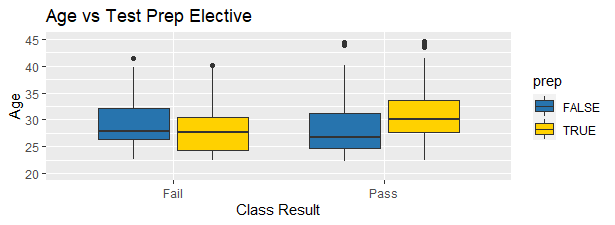
\includegraphics[width = \textwidth]{Plots/age_test_prep.png}
\end{center}

\subsubsection{Cultural Electives}

A similar model was used to predict whether a student wanted to enroll in a cultural course. Region was again an important predictor, in addition to a binary variable indicating whether the student wanted to enroll in a test prep course.

Students from the Middle East were 2.2 times as likely to take cultural courses than any other region. Students who wanted to enroll in a test prep course were 1.7 times as likely to also want to enroll in a cultural course (perhaps counter-intuitively, as each student had four courses to select and the groups would presumably be competing for enrollment). This is still a statistically significant predictor even after accounting for the region of the student. Age, gender, and grades do not appear to be a factor.

\subsubsection{Business English}

No demographics appear to be significantly related to wishing to enroll in Business English. However, other courses appear to be a factor. Specifically, students who want to take a test prep course were 1.9 times as likely to want to take Business English, and students who want to take a cultural course were 10.7 times as likely.

\begin{center}
    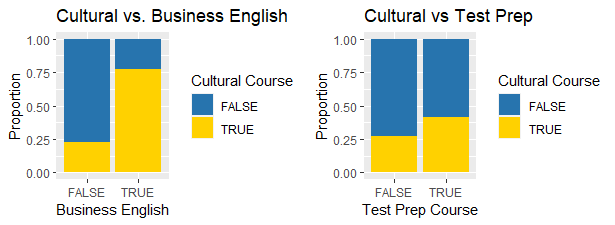
\includegraphics[width = \textwidth]{Plots/course_correlations.png}
\end{center}

\subsubsection{Relationship with Knowledge of American Culture}

The previous Stats 141XP students heavily analyzed which students self-identified as having improved their knowledge of American culture through taking a course. Perhaps unexpectedly, there does not appear to be any relationship at all between a willingness to enroll in cultural courses and having an improvement in knowledge of American culture.

\begin{center}
    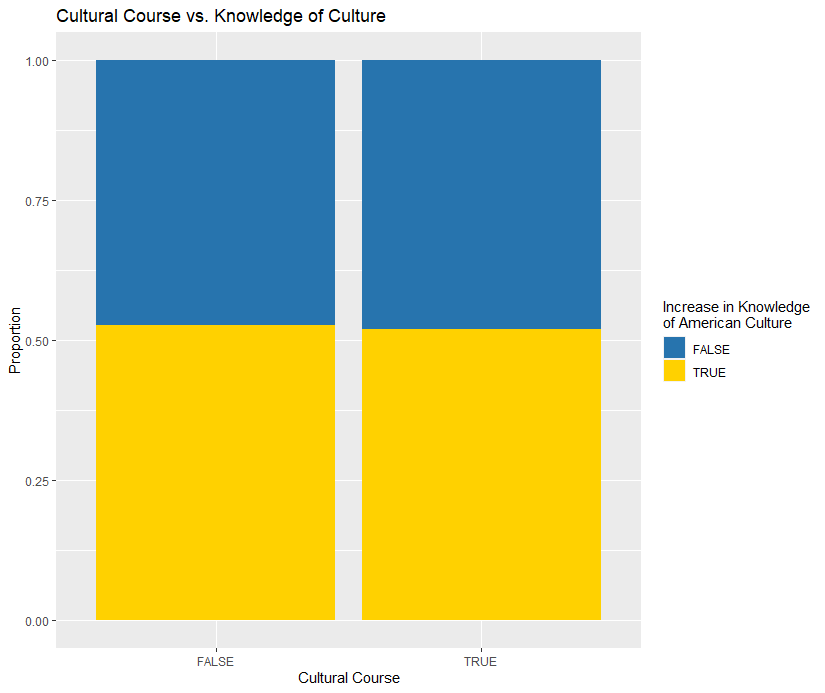
\includegraphics[width = \textwidth, height = 400]
    {Plots/lol_culture.png}
\end{center}


\subsection{Absences and Demographics}

For each student, three metrics of course results were measured. A pseudo-GPA metric was created, combining results from both letter-grade courses and Pass/No Pass courses. The average number of absences per course was measured for each student. Finally, a binary variable indicating whether the student failed at least one course was also created. As one would expect, the three results are highly correlated with each other.

\begin{figure}[!bp]
  \centering
  \begin{minipage}[b]{0.49\textwidth}
    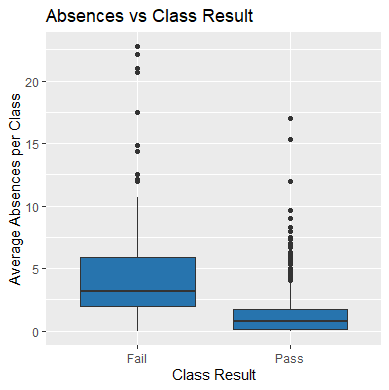
\includegraphics[width=\textwidth]{Plots/absence_fail.png}
  \end{minipage}
  \hfill
  \begin{minipage}[b]{0.49\textwidth}
    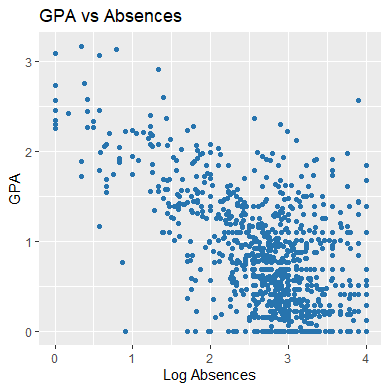
\includegraphics[width=\textwidth]{Plots/gpa_absences.png}
  \end{minipage}
\end{figure}

A multiple linear regression was performed to predict absences using demographic variables and other course result metrics. The important predictors were found to be the other two result metrics, as well as the region of the student. Other demographics, such as gender and age, were not important.

The differences between any pair of the three regions (Middle East, Asia, Other) were significant, as were their interaction effects with the indicator of whether the student failed a course. Among students that failed at least one course, the distribution of absences appears to be similar regardless of region. However, for those who have not failed a course, we viewed clear distinctions between region. Students from the Middle East tended to have the most absences, and students from Asia tended to have the least.

\begin{center}
    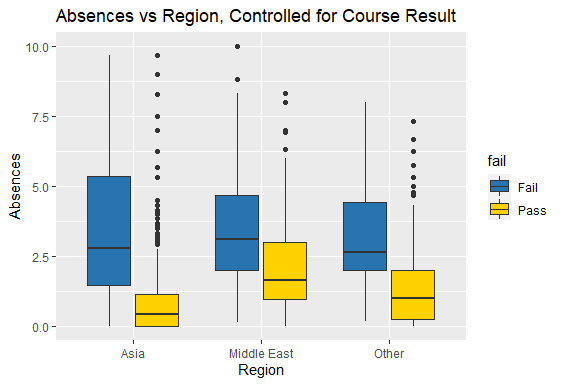
\includegraphics[width = \textwidth]{Plots/region_absences.png}
\end{center}

\newpage

%***RESULTS***%
\section{Results}

\subsection{Survey Score}

	Further analysis for replies to the multiple choice section of the survey was done using the Program Evaluation data. Each multiple choice survey question was answered from a selection of five answers with the first being the least happy and the fifth being the happiest with their experience. Some of these questions include “This teacher explains things clearly,” “My general evaluation of this course is,” and “How satisfied were you with the textbooks used in this course” among others. The replies were given a numeric value between one and five and then summed up to create the student’s survey score separated for each student by course schedule (Monday and Wednesday, Tuesday and Thursday, Monday and Thursday, etc.).
	
	Some examples of results include the 9 question evaluations of students with Tuesday and Thursday classes (a group of approximately 1000 students) where it was found that 73.9 percent of respondents had a survey score of 45 or 27. Additionally, in the 9 question evaluations of students with Monday and Wednesday classes (249 students) about 46.2 percent of students had a score of 45 or 27. For both of these cases the range was between 9 (all ones) and 45 (all fives). Overall, the survey score showed students often answer all 3s (middle value) or 5s (highest value). However, the score was not found to be a significant predictor of absences. 


\begin{figure}[!ht]
  \centering
  \begin{minipage}[b]{0.49\textwidth}
    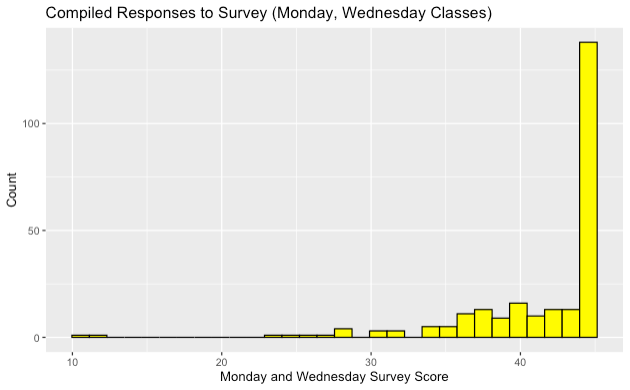
\includegraphics[width=\textwidth]{Plots/MW Survey Score.png}
  \end{minipage}
  \hfill
  \begin{minipage}[b]{0.49\textwidth}
    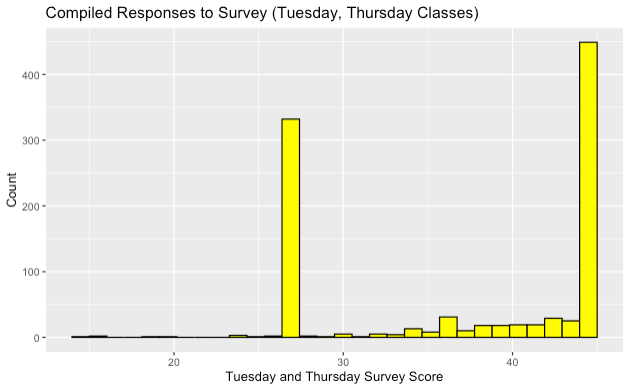
\includegraphics[width=\textwidth]{Plots/TTH Survey Score.png}
  \end{minipage}
\end{figure}


\subsection{Feature Selection Methodology}

We also wanted to see what other predictors were significant in predicting student absences other than grades and region. By doing so, we wished to able to form a more complete understanding of what groups of students tend to miss more classes than others. This will be able to motivate us to create recommendations as to how to possibly reduce these absences in the future. For our predictors, we have 22 further variables to analyze, including ones such as "ALC Initial Placement", New/Returning Student", "Plans", "Gender", "Preferred ZIP", "Instructor", "Cohort", among many others. 

For the methodology in determining which predictors were significantly associated with number of absences, we first began to do exploratory data analysis on absences with each of the different predictors through box plots. These plots gave us a general idea of how different each group is in regards to absences. However, there were some instances where the differences seemed too close from only looking at the plots and so we needed more quantitative methods in establishing statistical significance.

The next step is we utilized numerous statistical techniques and methods in filtering out which predictors were significant or not. Our main method was factor analysis on each of the 23 different predictors. However, we also implemented AIC/BIC subset selection, variable importance from random forest, and predictor shrinkage from LASSO regression. 

Then, after looking at all of the outputs from each of these different statistical techniques, we conducted post-hoc analysis on the predictors that, on average, were chosen by these different variable selection methods. This allowed us to see what specific pairwise differences were significant from each of the different groups or levels within each of the different selected predictors. By doing so, we gained further insight into the relationship between these variables and the number of absences.

The predictors that were not only significant with absences but also interesting to delve deeper into were "Placement Levels", "New/Returning Students", "AEIP Completion", "Payor", "Planned Field of Study", and "Hear About ALC".

\subsection{Relationships with Absences}

Factor analysis was conducted to analyze which predictors are the most significant in predicting absences, thus potentially generating a metric for engagement. It will also help us understand whether different characteristics of students will lead to certain patterns in absences. We looked at 23 different predictors, and the following are what we determined to be the most significant or interesting to analyze.

\subsubsection{Placement Levels}

First, we looked at placement levels of certain classes. From the boxplots, we were able to generalize that students in lower placement levels tend to have more absences. This is also consistent throughout different classes.

\begin{center}
    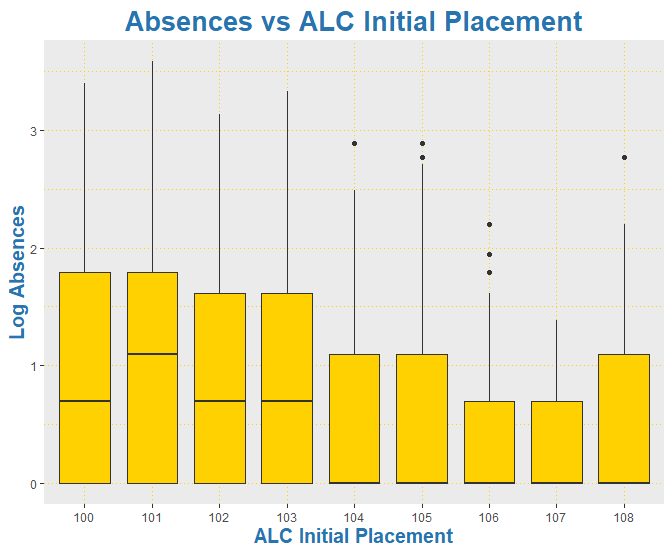
\includegraphics[width = 0.5\textwidth]{Plots/1. ALC Initial Placement.png}
\end{center}

\begin{figure}[!ht]
  \centering
  \begin{minipage}[b]{0.49\textwidth}
    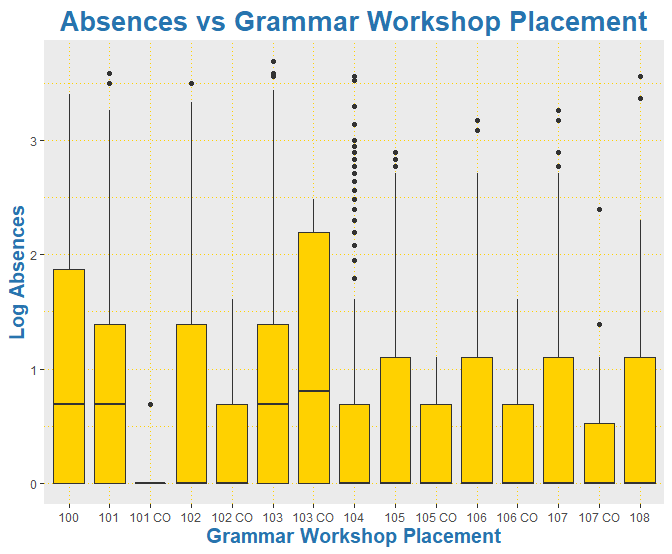
\includegraphics[width=\textwidth]{Plots/1. Grammar Workshop Placement.png}
  \end{minipage}
  \hfill
  \begin{minipage}[b]{0.49\textwidth}
    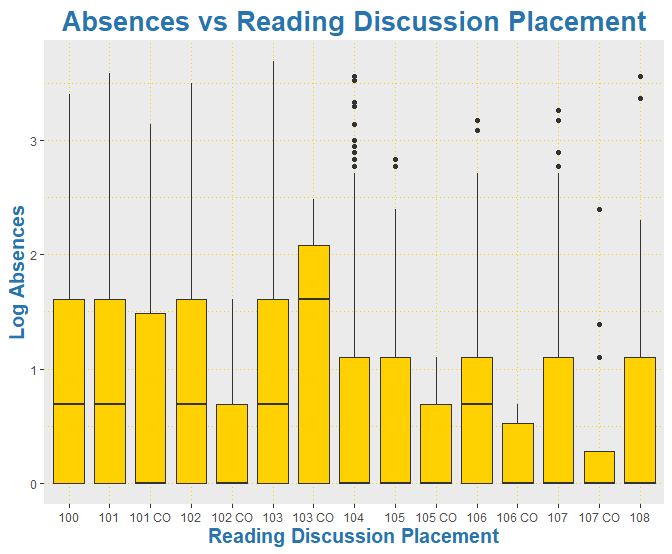
\includegraphics[width=\textwidth]{Plots/1. Reading Discussion Placement.png}
  \end{minipage}
\end{figure}

\subsubsection{New/Returning Students}

Next, we wondered whether there would be a difference in absences for new and returning students. The result was a significant difference in new and returning students. More specifically, returning students tend to have more absences than new students. This could potentially be because returning students are likely to relax a bit more in classes once they are settled in compared to new students who just enrolled in the program.

\begin{center}
    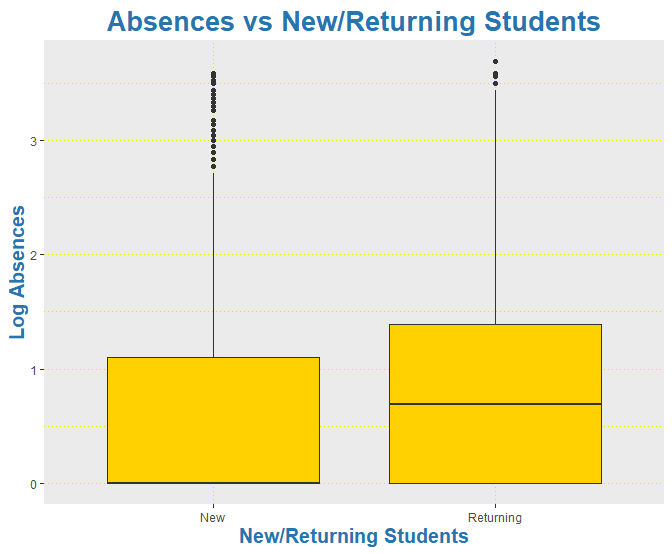
\includegraphics[width = 0.55\textwidth]{Plots/2. New Returning Students.png}
\end{center}

\subsubsection{AEIP Completion}

We can also see that students who cancelled, terminated, or withdrew from AIEP tend to have more absences in classes. This result is expected as students doing worse are also the students who miss more classes.

\begin{center}
    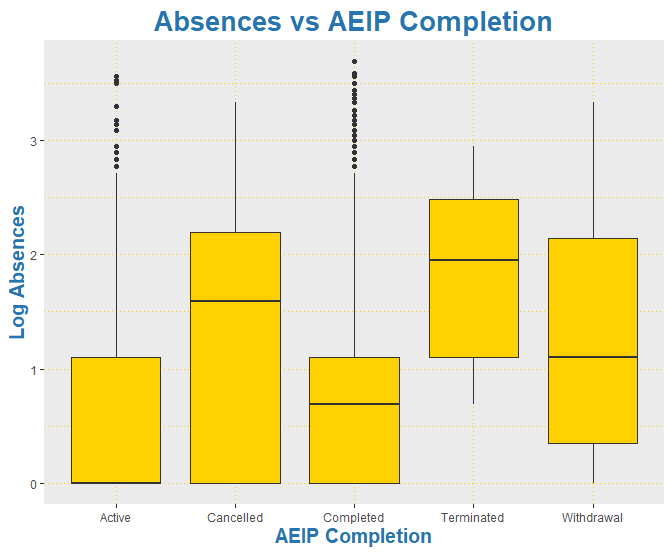
\includegraphics[width = 0.55\textwidth]{Plots/3. AEIP Completion.png}
\end{center}

\subsubsection{Payor}

The next three predictors offer significant differences, but based on the lack of differences in the median in boxplots and the large amount of data used, we must be careful with the conclusions that we arrive at. A significant difference may not necessarily mean a relationship where one group of students will indeed lead to more absences than another.

With that being said, we look at absences versus who paid for the students’ participation in the program. From the boxplot, we can see that there really is no difference between if it is family or self-funded, but there seems to be a larger amount of absences in "Other" payors. These include external scholarships from schools, organizations, or governments. After post-hoc analysis is conducted, it does indeed show that “Other” is significantly different from self or family payments. Though not extremely significant, it does offer insight into how students not funding their own program fees are likely to be less engaged with the program.

\begin{figure}[!ht]
  \centering
  \begin{minipage}[b]{0.49\textwidth}
    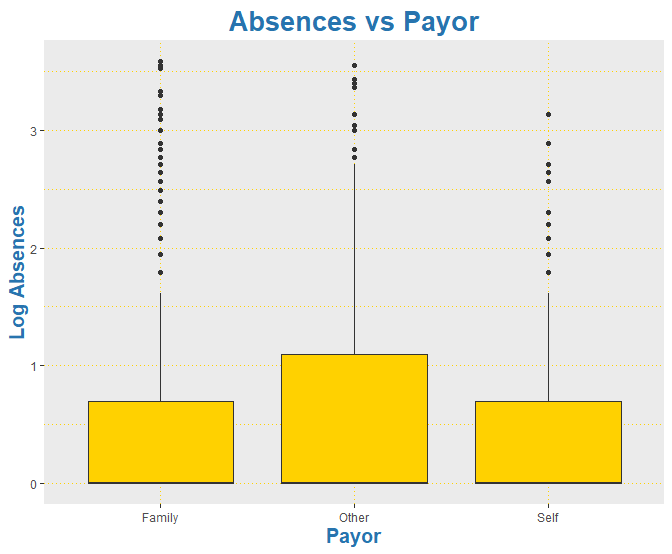
\includegraphics[width=\textwidth]{Plots/4. Payor.png}
  \end{minipage}
  \hfill
  \begin{minipage}[b]{0.49\textwidth}
    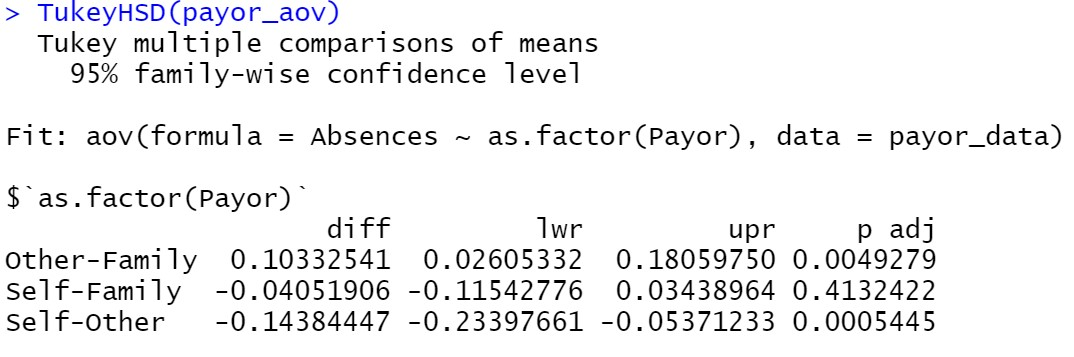
\includegraphics[width=\textwidth]{Plots/4. Payor Tukey.jpg}
  \end{minipage}
\end{figure}

\subsubsection{Planned Field of Study}

Another variable we looked at is what students plan to study after. After conducting post-hoc, we can see that STEM students tend to miss more classes on average than Humanities students, and the result is significant. It could be because STEM students typically would prefer more math-based or number-based classes instead of language-based classes.

\begin{figure}[!ht]
  \centering
  \begin{minipage}[b]{0.49\textwidth}
    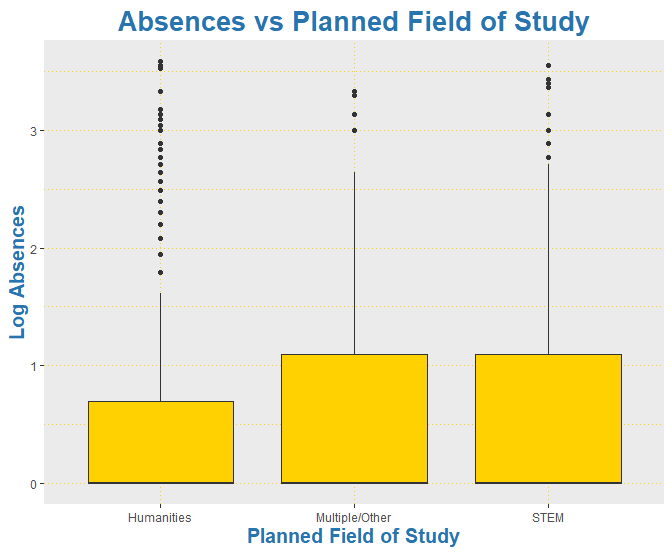
\includegraphics[width=\textwidth]{Plots/5. Planned Field.png}
  \end{minipage}
  \hfill
  \begin{minipage}[b]{0.49\textwidth}
    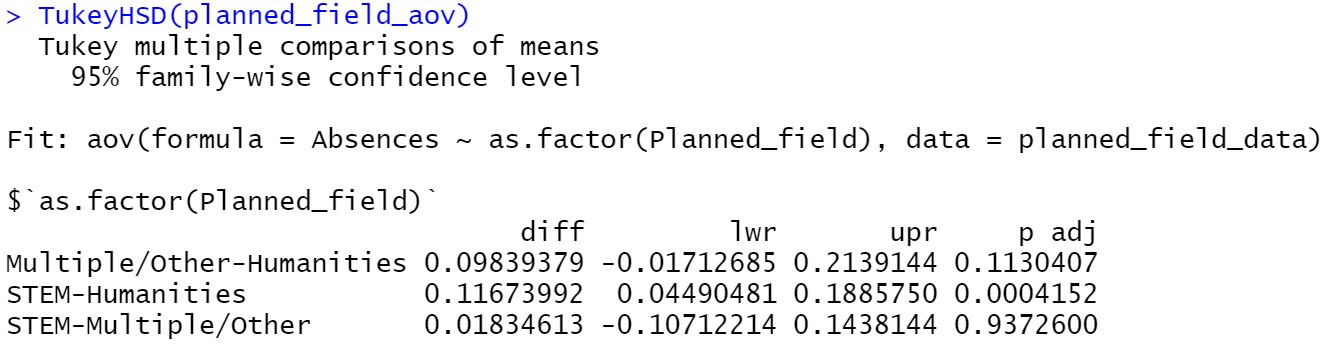
\includegraphics[width=\textwidth]{Plots/5. Planned Field Tukey.jpg}
  \end{minipage}
\end{figure}

\subsubsection{Hear About ALC}

Another interesting variable we looked at is how the students heard about ALC. It seems like students who heard about the program from family or friends tend to miss more classes than if students hear about it from the Internet. Post-hoc also shows a significant difference between family/friend and the internet. Intuition-wise, this might be because students who hear about ALC from family or friends might have enrolled in the program because of them, instead of their own choice, and students who looked up the program on their own time through the Internet tend to miss fewer classes and be more engaged because it is of their own will and interest. 

\begin{figure}[!ht]
  \centering
  \begin{minipage}[b]{0.49\textwidth}
    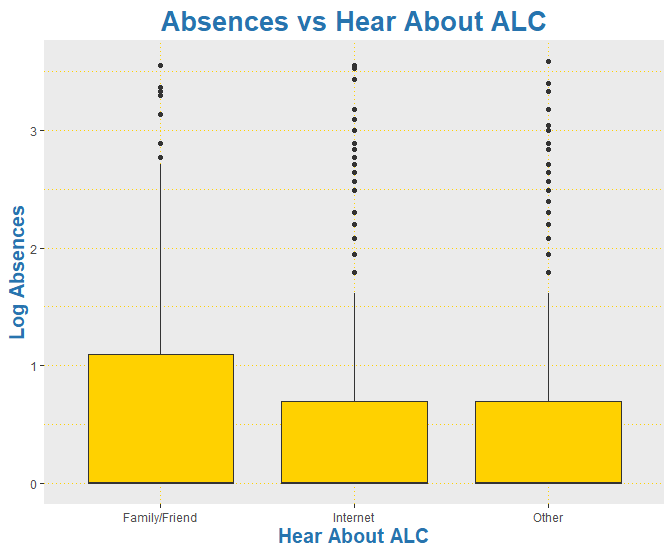
\includegraphics[width=\textwidth]{Plots/6. Hear About ALC.png}
  \end{minipage}
  \hfill
  \begin{minipage}[b]{0.49\textwidth}
    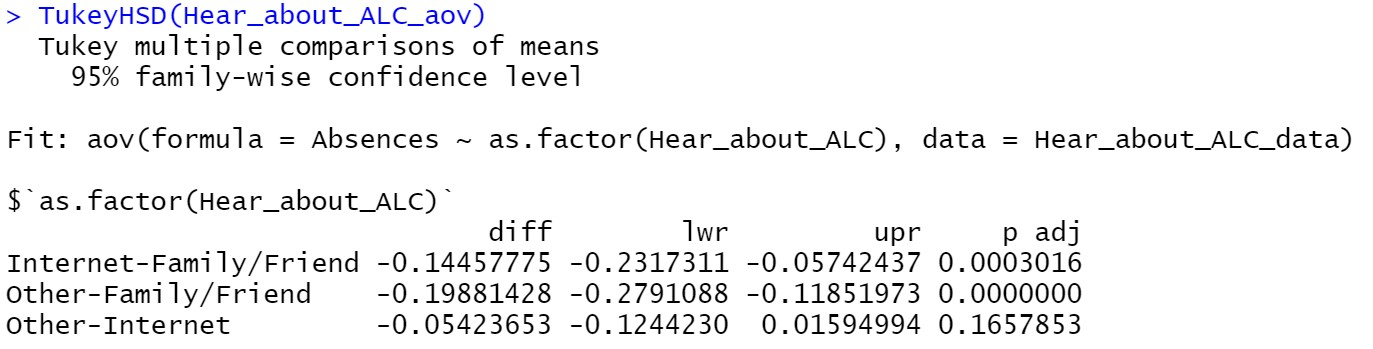
\includegraphics[width=\textwidth]{Plots/6. Hear About ALC Tukey.jpg}
  \end{minipage}
\end{figure}

\newpage

%***CONCLUSION***%
\section{Conclusion}

\subsection{Overall Conclusions}

We found the Region variable to be one of the most important factors in predicting course outcomes as well as elective course preferences. Additionally, we found that students who prefer to take Test Prep courses also prefer to take Cultural and Business English courses. One of our most significant findings concerning engagement was that new students in the program are more likely to have fewer absences than returning students. Furthermore, we found that students who heard about the program through the Internet tend to miss fewer classes as opposed to word-of-mouth.

\subsection{Challenges}

The most significant challenge during this project was handling missing data. There was a lack of shared student IDs between data frames and file types. We solved this partially through combining the observations of every file in each of the file types in order to create a single cohesive data set for analysis. Unfortunately, many survey questions had missing values, even if excluding the program evaluations. Because removing all observations with missing values would leave us with an empty data set, we recoded the missing values as their own category for categorical variables. Similarly, lack of free responses from students on teachers, courses, and programs impeded our ability to conduct meaningful sentiment analysis.

\subsection{Recommendations}

Given the results of the study, the two main recommendations would most likely have to be first, studying how the predictors found to be significant with engagement in turn relate to the demographic variables and, second, identifying the demographics of the students that are most engaged and are relatively underrepresented to help improve the marketing efforts. For future studies, it could be valuable to analyze survey design as well as the interactions between survey questions, specifically better ways of conducting surveys, developing a consistent and unchanging set of effective and unbiased questions, or even interviewing students. Students would also be more inclined to give honest, thorough answers if given an in-class incentive to finish the course evaluation.

%***Thank the Professor section***%
\section{Acknowledgements}

Special thanks to Professor Esfandiari for teaching us the necessary material to do the project, to Professor Thomas for giving us the unique opportunity to apply our statistical skill-sets to real world problems, and to Sam for always being there for us. :)


\pagebreak


 

\end{document}